

In the proposed architecture, the \textit{Smart Gateway} is the central module of the system, connecting the \textit{SmartBoxes} to the \acs{HIS}. It is responsible for the management of devices and their associations -- \textit{SmartBox} to \textit{Biosticker} and \textit{SmartBox} to user -- managing, maintaining and storing the data that is generated by these, as well as handling any communication to and from the \acs{HIS}. 


\paragraph{} Regarding the hardware platform used for the \textit{Smart Gateway}, in the context of the \acs{WoW} project, we use the Intel NUC NUC8i7BEH\footnote{Intel NUC NUC8i7BEH product page: \url{https://ark.intel.com/content/www/us/en/ark/products/126140/intel-nuc-kit-nuc8i7beh.html}}.

\begin{figure}[H]
    \centering
    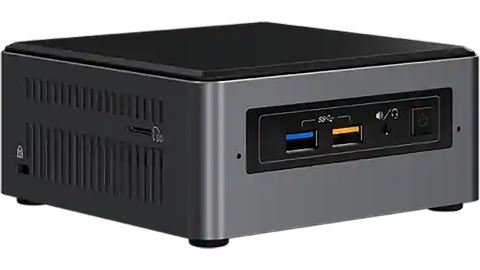
\includegraphics[width=0.4\linewidth]{images/gateway-image.png}
    \caption[Intel NUC NUC8i7BEH.]{Intel NUC NUC8i7BEH.}
    \label{fig:gateway_image}
\end{figure}


\paragraph{} In the next sections, we propose a service architecture for the \textit{Smart Gateway} in order to fulfill the aforementioned features.

% The \textit{Smart Gateway} maintains a list of all the \textit{SmartBoxes} that are managed by the system, as well as every \textit{Biosticker} and every sensor in the \textit{Biosticker} (which are used to indicate respective biosignal to the \acs{HIS}). 


\section{Service Architecture}

As we have seen, there are multiple key features that form the \textit{Smart Gateway}. From Figure \ref{fig:wow-architecture}, we can list the different \textit{Smart Gateway} components:  

\begin{itemize}
    \item \textbf{Manage devices and device associations}: The \textit{Smart Gateway} maintains a list of all the \textit{SmartBoxes} that are managed by the system, as well as every \textit{Biosticker} and every sensor in the \textit{Biosticker} (which are used to indicate the respective biosignal to the \acs{HIS}). The \textit{Smart Gateway} also tracks the sensor subscriptions per \textit{SmartBox}.
    \item \textbf{Data anonymization}: Any private data (\textit{i.e.} information that can be used to identify a user) that is stored in the \textit{Smart Gateway} is anonymized in order to meet data protection regulations\footnote{Resolution of the Council of Ministers no. 41/2018, of 28 March, following the new General Data Protection Regulation (GDPR), approved by Regulation (EU) 2016/679:  \url{https://dre.pt/application/file/a/114936962\%20}}. 
    \item \textbf{Data pre-processing}: The \textit{Smart Gateway} processes the data as it is collected in order to clean the data before storing it indefinitely, and to detect critical conditions of the patients' state to prompt an immediate notification to the health professionals.
    \item \textbf{Real-time data acquisition}: The \textit{Smart Gateway} handles the secure communications with the \textit{SmartBoxes}, acquiring the data in real-time.
    \item \textbf{Manage data collection}: After receiving and processing the data from the \textit{SmartBoxes}, the \textit{Smart Gateway} stores indefinitely for long-term biomonitoring analytics.
    \item \textbf{\acs{HIS} \acs{FHIR} Integration}: The \textit{Smart Gateway} handles the communication with the \acs{HIS}. More specifically, it processes all \acs{FHIR} requests from the \acs{HIS}, and also transforms the acquired sensor data into \acs{FHIR} messages and communicates it to the \acs{HIS}. 
\end{itemize}

To implement these components, we propose the following service architecture within the \textit{Smart Gateway}, as illustrated on Figure \ref{fig:gateway_serviceoverview}. The correspondence between the services and the \textit{Smart Gateway} components is described in Table \ref{tab:gateway-service}.

\begin{figure}[H]
    \centering
    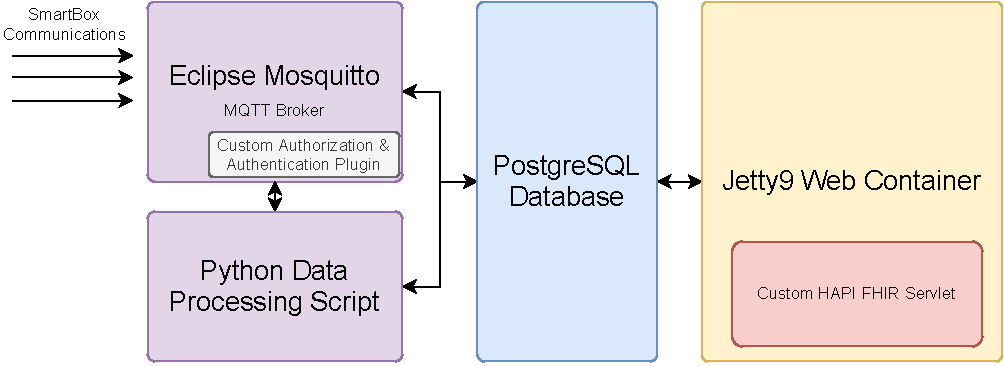
\includegraphics[width=0.8\linewidth]{images/service overview gateway.pdf}
    \caption[Service architecture implemented in the \textit{Smart Gateway}.]{Service architecture implemented in the \textit{Smart Gateway}. The diagram displays the different technologies used throughout the development. The services communicate with each other using Unix Domain Sockets, a Linux protocol for \acf{IPC}.}
    \label{fig:gateway_serviceoverview}
\end{figure}
\begin{table}[]
    \caption{Correspondence between the \textit{Smart Gateway} services and its functional components.}
    \label{tab:gateway-service}
    \resizebox{\textwidth}{!}{%
    \begin{tabular}{ccc}
    \hline
    \textbf{\textit{Smart Gateway} Component}          & \textbf{\textit{Smart Gateway} Service} & \textbf{Description}                                                                                                                                                             \\ \hline
    Real-time data acquisition             & MQTT Broker                   & \makecell[c]{This service is responsible for handling all the\\  \textit{SmartBoxes} communication, ensuring data\\  encryption, authorization, etc.}                                                           \\ \hline
    Data pre-processing                    & Data processing               & \makecell[c]{This service is handles data filtering and \\ preliminary data processing.}                                                                                                  \\ \hline
    \multirow{3}{*}{\makecell[c]{Manage data collection \\ Manage devices and device associations}}                & \multirow{3}{*}{Data storage} & \multirow{3}{*}{\makecell[c]{This service manages and stores system information,\\ such as the list of devices, permissions of each \\ device and collected sensor data.}} \\
     &                               &                                                                                                                                                                                  \\ & & \\ \hline
    Data anonymization                     & \multirow{2}{*}{FHIR Server}  & \multirow{2}{*}{\makecell[c]{This service is responsible for handling communications \\with the  ``Interoperability'' layer  of \acs{HIS}.}}                                                         \\ 
    \acs{HIS} \acs{FHIR} Integration       &                               &              \\\hline                                                                                                                                                                   
    \end{tabular}
    }
\end{table}

\paragraph{} The services communicate with one another using UNIX Domain Sockets\footnote{\url{https://man7.org/linux/man-pages/man7/unix.7.html}}. This is an interprocess communication (\acs{IPC}) protocol that enables efficient communication between processes running on the same host operative system. This protocol is very efficient, compared for example to traditional network sockets \cite{Wright2007}, since all communication is handled entirely by the operative system kernel, instead of relying on \acs{IP} protocol stack, minimizing communication overhead. 

The protocol can make use of the Linux file system for addressing, which means it is subject to Linux file system permissions. This allows applications to identify which process, or more accurately, the user running the process, is attempting to establish a new connection to that application, providing a simple and secure authentication mechanism on the \acs{IPC}.

\section{Data Storage}

The data storage in the \textit{Smart Gateway} is one of the most important components of the device, as it holds the information used by all services in the \textit{Smart Gateway}. Given the importance of this component, it is crucial to use a solution which offers reliability above all, with proved performance for our use case.  

\paragraph{} As discussed in Section \ref{sec:iot-model-layer4}, No\acs{SQL} databases are appealing for \acs{IoT} applications, since these can handle unstructured or semi-structured data and generally better performance than traditional \acs{SQL} databases as the amount of data stored increases. For our use case, 

\paragraph{}

We find that PostgreSQL has a respectable performance, even beating No\acs{SQL} databases like MongoDB 


%\cite{Asiminidis2018} 

\paragraph{} PostgreSQL\footnote{\url{https://www.postgresql.org}} is an advanced, enterprise-class, and open-source \acs{RDBMS}. It has over 30 years of active development by the open source community, earning a strong reputation for its reliability, feature set and robustness.

\footnote{DB-Engines Monthly Popularity Ranking: \url{https://db-engines.com/en/ranking}}


% it is important to choose a solution which offers availability

% PostgreSQL offers a balance between \footnote{\url{https://itnext.io/benchmark-databases-in-docker-mysql-postgresql-sql-server-7b129368eed7?gi=a506815fb197}}

\subsection{Database Schema}
Figure \ref{fig:wow-dbschema-full} contains the database model implemented in our PostgreSQL database. It describes all information that is contained in the \textit{Smart Gateway}, the relations within that data, organized according to the functionality it is related to, which will be explored in greater detail in the next sections.

\begin{figure}[H]
    \centering
    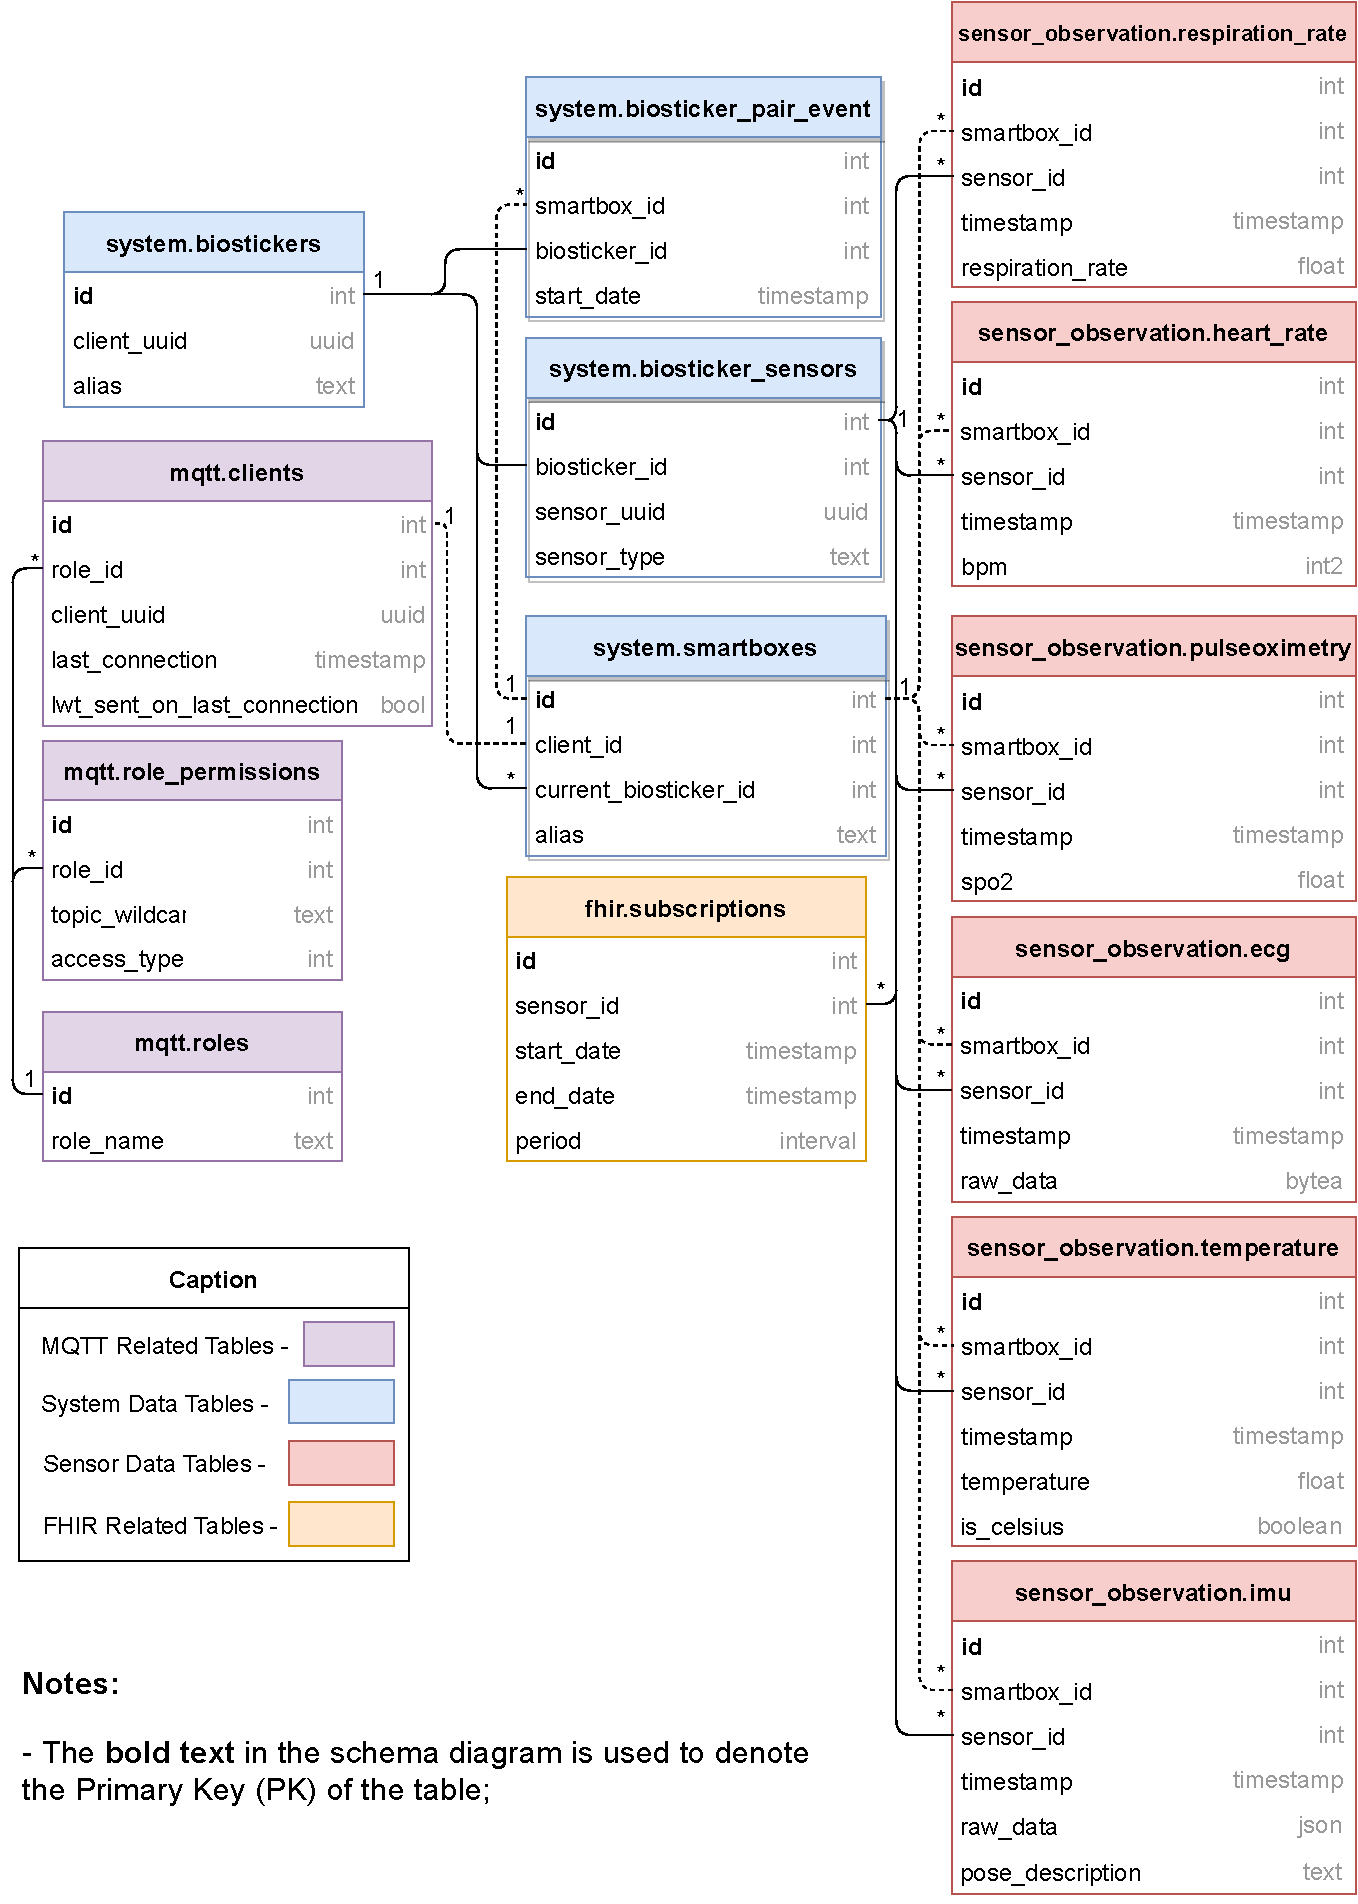
\includegraphics[width=0.9\linewidth]{images/database-schema-general.pdf}
    \caption[Database schema implemented in the \textit{Smart Gateway}.]{Database schema implemented in the \textit{Smart Gateway}. The bold text in the schema diagram is used to denote the Primary Key (PK) of the table. The relationships between the entities are indicated using the symbol ``*'' for many and ``1'' for one in the graph.}
    \label{fig:wow-dbschema-full}
\end{figure}

\subsubsection{MQTT Client Information}

Figure \ref{fig:wow-dbschema-mqtt} contains the information relevant for \acs{MQTT} communications, mostly related with security. To ensure that each device only has access to its own resources, the system implements a \acf{RBAC} policy. 
In this type of access control, the system allows and revokes access to resources according to the role of the device. 

\paragraph{} In context of the \acs{WoW} project, the following roles are used:

\begin{itemize}
    \item \textit{SmartBox} role: Indicates the \acs{MQTT} client is a \textit{SmartBox}.
    \item ``Pyservice'' role: Indicates the \acs{MQTT} client is actually the data processing service, also contained in the \textit{Smart Gateway}.
    \item Developer device role: Indicates the \acs{MQTT} client is a developer device, used solely for debugging purposes.
\end{itemize}


\begin{figure}[H]
    \centering
    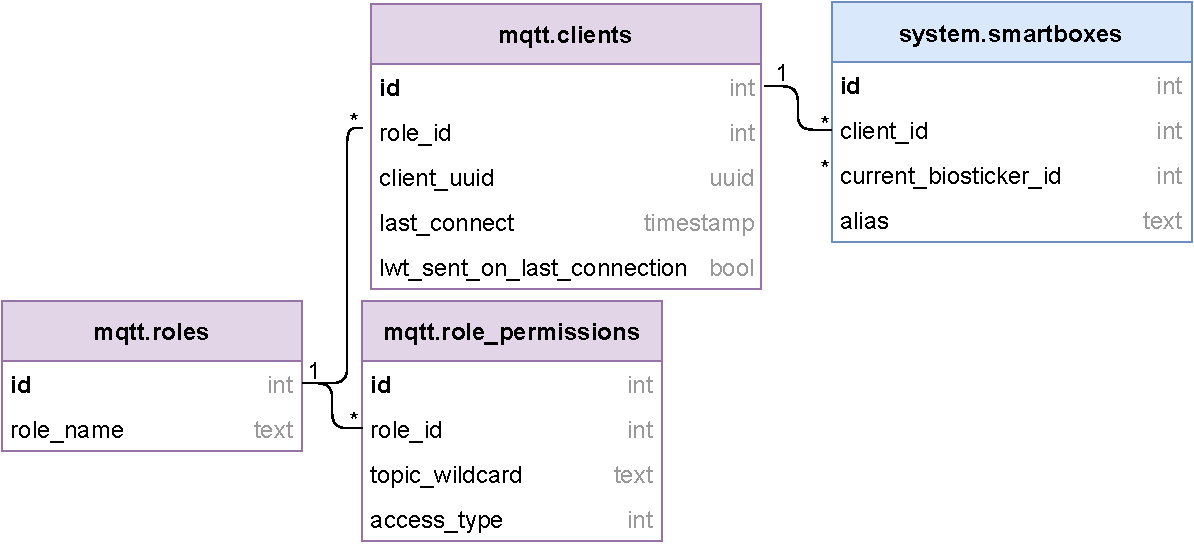
\includegraphics[width=\linewidth]{images/database-schema-mqtt.pdf}
    \caption[\acs{MQTT} information in the schema implemented in the \textit{Smart Gateway}.]{\acs{MQTT} information in the schema implemented in the \textit{Smart Gateway}.
    The ``mqtt.roles'' table contains the different \acs{RBAC} roles for the \acs{MQTT} communication and ``mqtt.role\_permissions'' table lists the permissions available to each role using \acs{MQTT} topic wildcards. The ``mqtt.client'' table lists the clients and their properties, such as their \acs{UUID}, the timestamp of their last connection, or a \textit{flag} to indicate if the communication failed during the last communication.
    
    }
    \label{fig:wow-dbschema-mqtt}
\end{figure}

\subsubsection{Sensor Data}

Figure \ref{fig:wow-dbschema-sensors} contains the sensor data collected over time. The tables 

\begin{figure}[H]
    \centering
    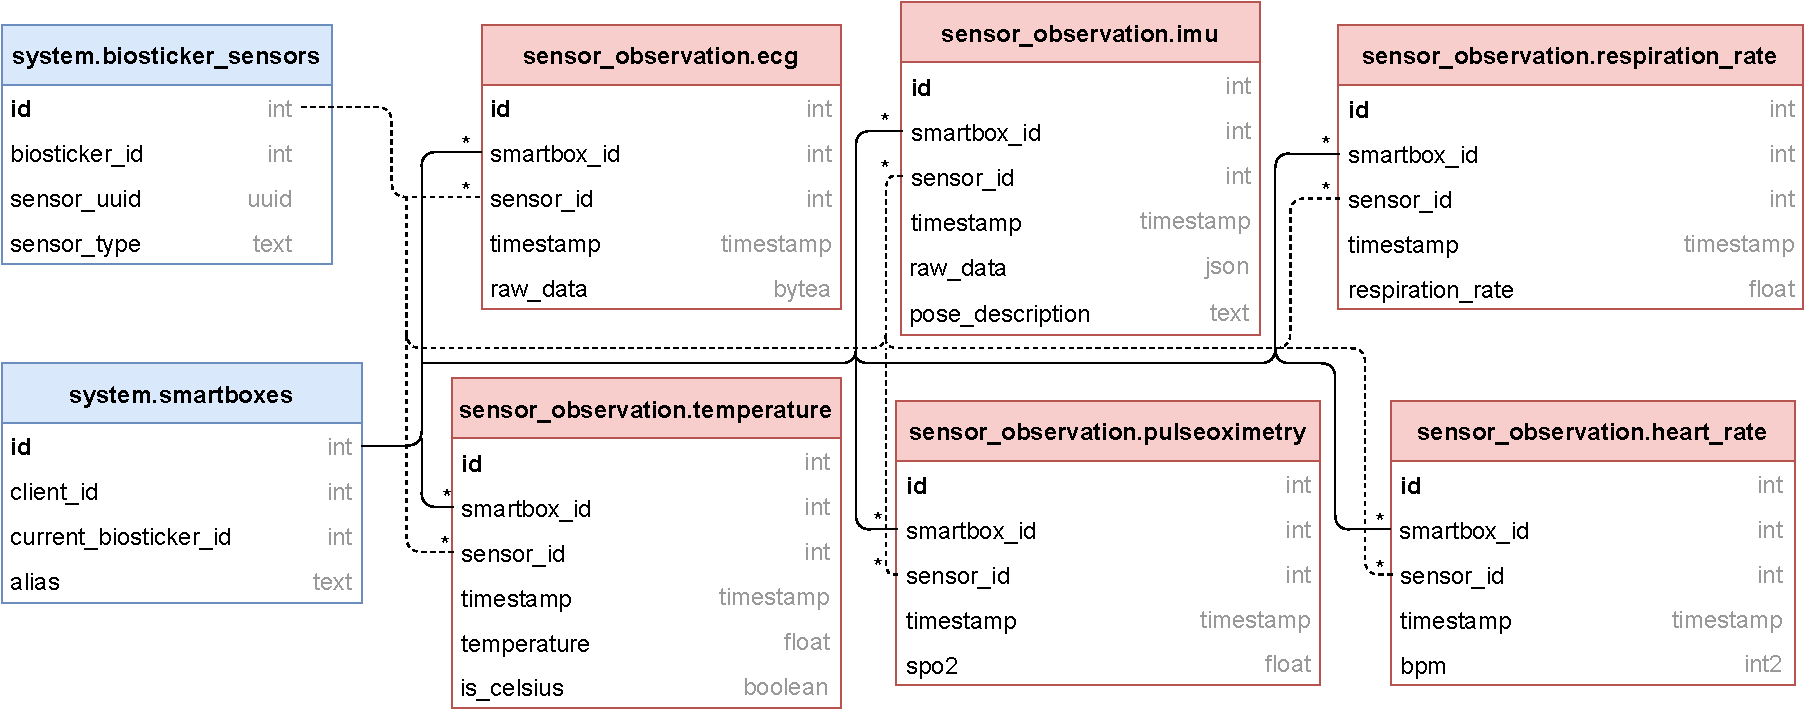
\includegraphics[width=\linewidth]{images/database-schema-sensordata.pdf}
    \caption[Sensor data information in the schema implemented in the \textit{Smart Gateway}.]{
        Sensor data information in the schema implemented in the \textit{Smart Gateway}. Our database model has one table for each different type of biosignal (temperature, \acs{ECG}, etc.). The properties of the table are defined according to the data acquired on the \textit{SmartBox} level, which are detailed in Section \ref{sec:biosticker_data}.}
    \label{fig:wow-dbschema-sensors}
\end{figure}

\subsubsection{FHIR Related Information}
\dots 

\begin{figure}[H]
    \centering
    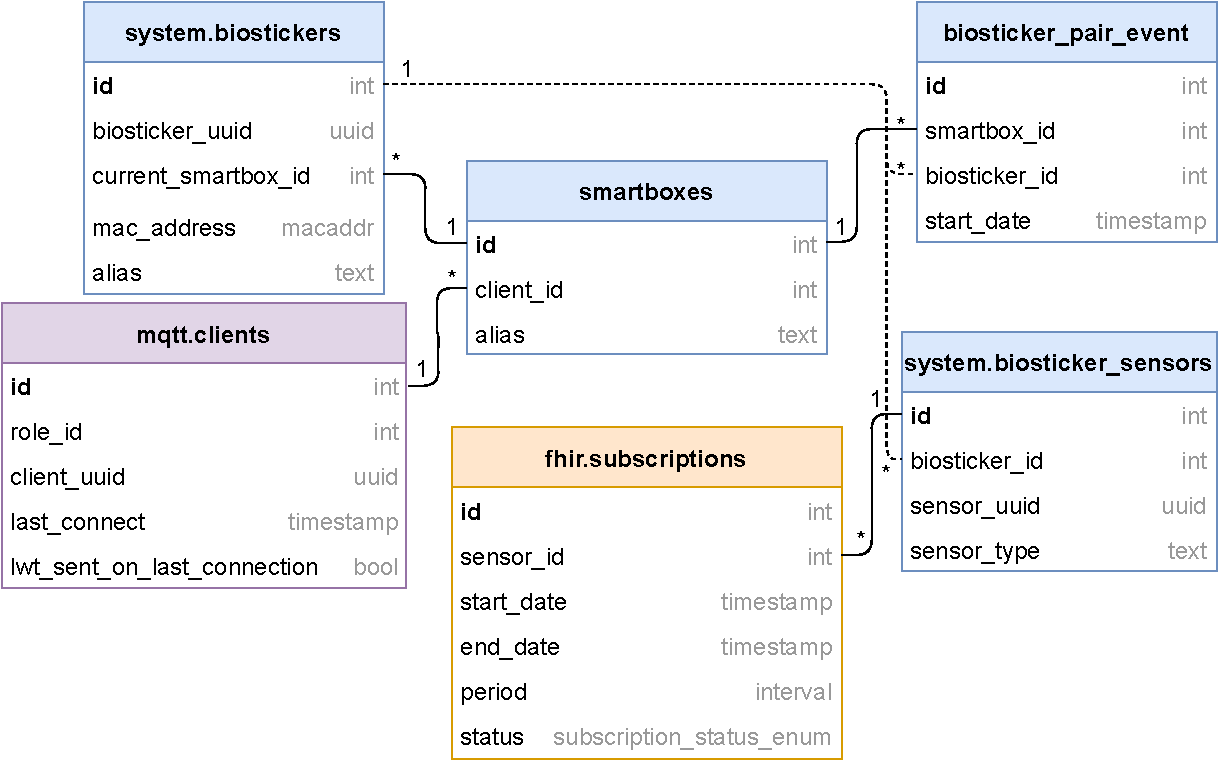
\includegraphics[width=\linewidth]{images/database-schema-fhir.pdf}
    \caption[test]{test}
    \label{fig:wow-dbschema-fhir}
\end{figure}
 

\subsubsection{Stored Procedures}

Since the \textit{Smart Gateway} makes use of a \acs{RDBMS}, services that access the database use \acf{SQL} to perform requests, such as retrieving data or inserting data. In order to maximize the performance of our data storage solution, we implemented ``Stored Procedures'', which are subroutines that are stored in the \acs{RDBMS}. These procedures are pre-compiled \acs{SQL} statements that are defined in the \acs{RDBMS}, and can greatly improve the performance of these systems since these:

\begin{itemize}
    \item Reduce significantly the amount of data that is exchanged -- instead of sending a request with a complex \acs{SQL} query to the database, the application sends a request for the execution of a subroutine along with its parameters, thus reducing the size of the request and the time it takes to interpret it.
    \item Reduce significantly the amount of data that is exchanged -- as these \acs{SQL} statements are optimized when pre-compiled.
    \item Increase the security and robustness of the database system -- since the \acs{SQL} statements are pre-compiled, this mitigates possible \acs{SQL} injections attacks\cite{clarke2012sql}, and also providing us with the ability to restrict the permissions of the applications that access the \acs{RDBMS} to execute only certain subroutines, instead of allowing them to perform general \acs{SQL} requests.
\end{itemize}


\section{Connection to the SmartBoxes}

As previously mentioned, the connection to the \textit{SmartBoxes} is performed via \acs{MQTT}. \acs{MQTT} is a centralized protocol, in which the clients (\textit{SmartBoxes}) connect to a broker, which acts as a middle-man for the communication, managing the requests from all clients accordingly. In our system, the broker is contained within the \textit{Smart Gateway}, and is the service responsible for ensuring the communication between the \textit{SmartBoxes} and our \acs{IoT} system.

\paragraph{} To implement this \acs{MQTT} broker, we use the open-source Eclipse Mosquitto\footnote{Eclipse Mosquitto -- An open-source \acs{MQTT} broker: \url{https://mosquitto.org/}}. Mosquitto is a lightweight \acs{MQTT} broker that supports the \acs{MQTT} protocol versions 5.0, 3.1.1 and 3.1 and is widely used by the community, making it a fitting solution for the \acs{WoW} project.

\paragraph{} Additionally, to define the intricacies of the \acs{MQTT} communication between the \textit{SmartBox} and \textit{Smart Gateway}, we propose a complete specification,detailing the security measures implemented, the format for the messages exchanged in the communication and the different endpoints used for 

full specification was proposed 

\subsection{Security}


\subsection{Authorization and Authentication Plugin}

One of the major flaws of Mosquitto is that it does not supply dynamic authentication and authorization processes for the \acs{MQTT} communication out-of-the box. By default, the list of \acs{MQTT} clients and their permissions are static, defined by a configuration file at the start of the program. In order to implement proper security measures, we developed a custom plugin using the extensive plugin \acs{API} \footnote{\url{https://mosquitto.org/api/files/mosquitto_plugin-h.html})} that implements authorization and authentication in the communications.

\paragraph{} The plugin works by intercepting authorization and authentication requests from the \acs{MQTT} broker, and validating the information in them. 

Whenever a \acs{MQTT} client sends a request to the broker -- connection request, subscription request or a publish request --, Mosquitto validates if the 

\todo[inline]{To-do: Add a flux diagram explaining how the authorization and authentication requests are handled.}


\section{Integration with GlobalCare}

- Mini introdução ao FHIR;
- mencionar camada de interoperabilidade da globalcare;
- indicar que optou-se usar HAPI devido ao facto de ser uma iniciativa open-source suportada por uma empresa de software hospitalar de renome.
- HAPI FHIR é baseada em Java servlets, fazer mini introdução do que são servlets e explicar o porquê de usar Jetty para correr servlets (é um web container, cujo objetivo é correr servlets). 

\subsection{FHIR Server}

- Falar do que são os FHIR Resources, e mais especificamente dos Resources usados para transmitir os dados -> Bundle, Device, Observation
- Apresentação do diagrama de comunicação de informação

\section{Summary}

In this chapter, we presented the different components which form the \textit{Smart Gateway}. In the chapter, we evaluate the performance of our proposed solution through a hospital trial.